% !TEX root = ../om_ts_06.tex

\begin{frame} % название фрагмента

\videotitle{ADF тест}

\end{frame}



\begin{frame}{ADF тест: план}
  \begin{itemize}[<+->]
    \item Предположения теста.
    \item Алгоритм теста.
    \item Три вариации теста.
  \end{itemize}

\end{frame}


\begin{frame}
  \frametitle{Зачем нужен ADF тест?}

  Хотим ответить на вопросы:
  \pause
  \begin{itemize}[<+->]
    \item Использовать $ARMA$ модель для $(y_t)$ или для $(\Delta y_t)$?
    \item Как включать константу в модель?
  \end{itemize}

  \pause
  Название «тест на единичные корни»:
  \pause
  \[
  \Delta = 1 - L = P(L) 
  \]
  Уравнение $1 - \ell = 0$ имеет корень $\ell =1$.

\end{frame}

\begin{frame}
  \frametitle{ADF тест}
  
  \begin{block}{Расшифровка}
    Augmented Dickey Fuller test
    
    Расширенный тест Дики-Фуллера  
  \end{block}

  \pause 
  Три вариации теста: без константы, с константой, c трендом.
  
\end{frame}


\begin{frame}
  \frametitle{ADF с константой}
  \[
  \Delta y_t = c + \beta y_{t-1} + d_1 \Delta y_{t-1} + \ldots + d_p \Delta y_{t-p} + u_t,  
  \]

  \pause

  \alert{$H_0$: $\beta = 0$};
  
  $(\Delta y_t)$ — стационарный $AR(p)$ процесс;

  $y_t = y_0 + mt + \sum_{i=1}^t (\Delta y_i - \E(\Delta y_i))$;

  \pause

  \alert{$H_a$: $\beta < 0$};

  $(y_t)$ — стационарный $AR(p + 1)$ процесс;

\end{frame}

\begin{frame}
  \frametitle{ADF с константой: $H_0$ и $H_a$}
  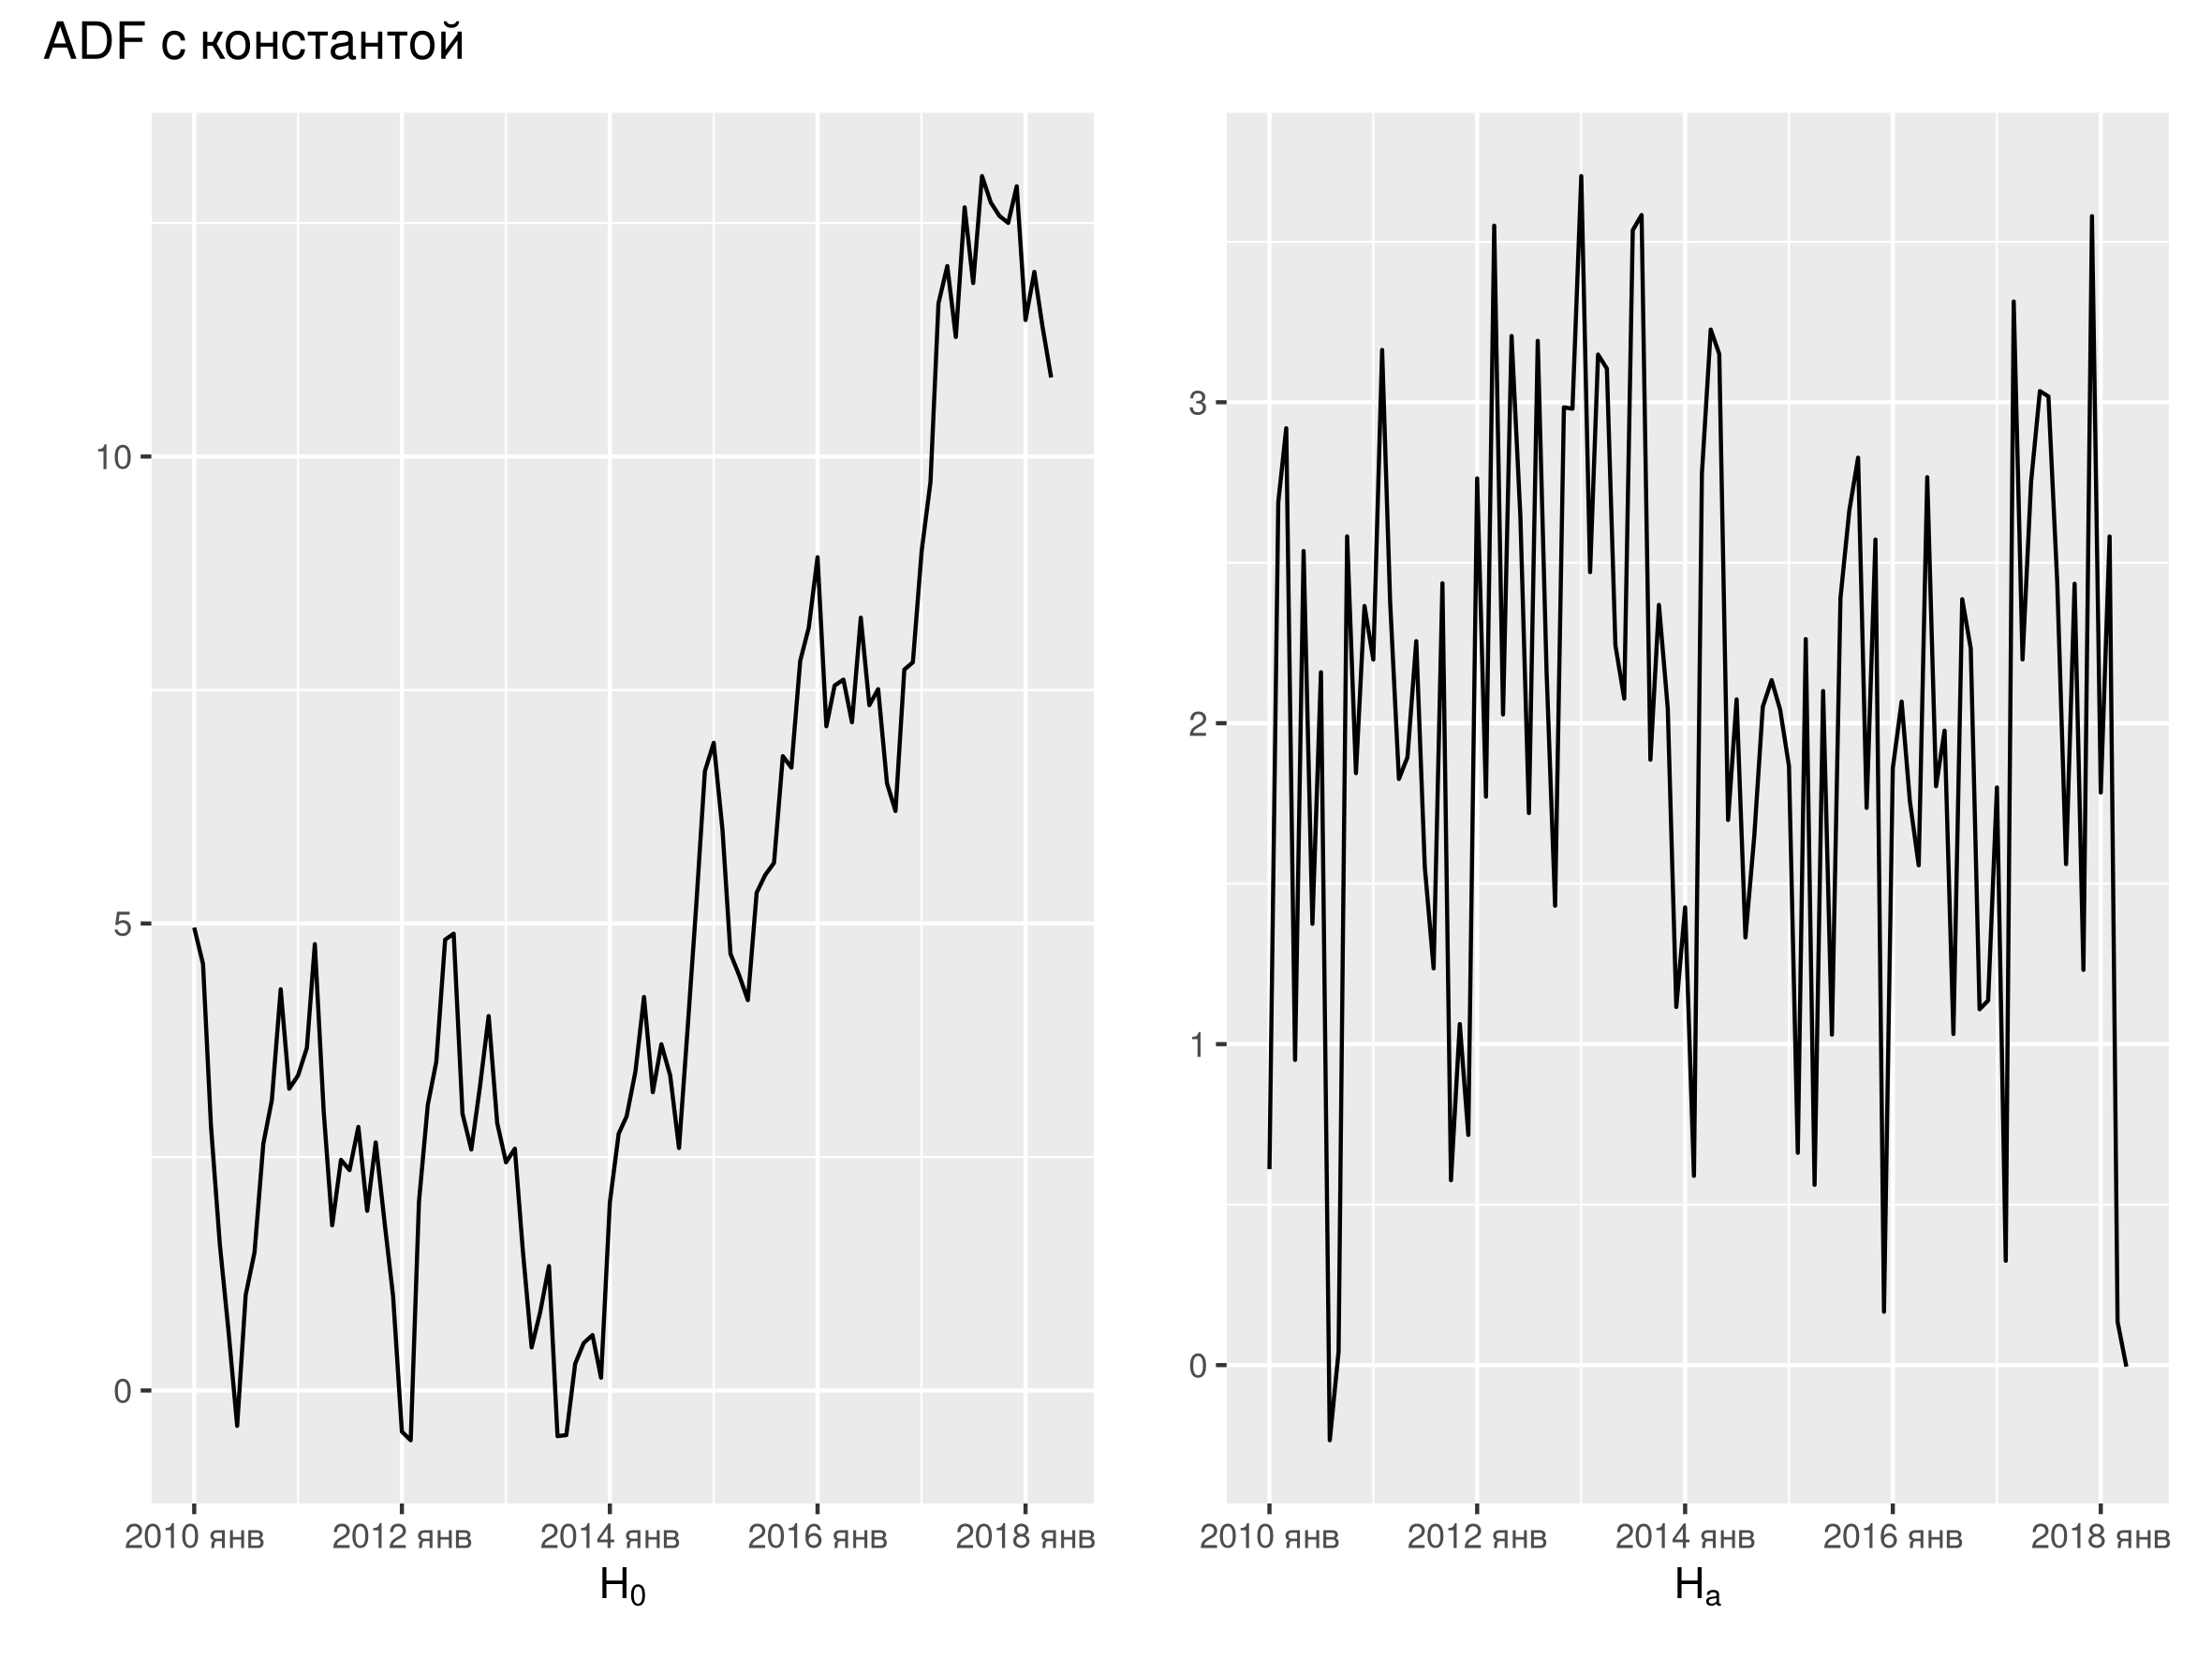
\includegraphics[width=\textwidth]{pictures/om_ts_06-046.png}

\end{frame}

\begin{frame}
  \frametitle{ADF с константой: алгоритм}

  Шаг 1. Оцениваем \alert{регрессию}
  \[
    \widehat{\Delta y_t} = \hat c + \hat \beta y_{t-1} + \hat d_1 \Delta y_{t-1} + \ldots + \hat d_p \Delta y_{t-p}.  
  \]

  \pause
  Шаг 2. Считаем по \alert{классической формуле} $t$-статистику
  \[
  ADF = \frac{\hat \beta -  0}{se(\hat \beta)}.  
  \]

  \pause
  При верной $H_0$ распределение $ADF$-статистики стремится к \alert{особому распределению} $DF^c$!

  \pause 
  Шаг 3. Делаем вывод:
  
  Если $ADF < DF^c$, то $H_0$ отвергается. 

\end{frame}


\begin{frame}
  \frametitle{ADF без константы}
  \[
  \Delta y_t = \beta y_{t-1} + d_1 \Delta y_{t-1} + \ldots + d_p \Delta y_{t-p} + u_t,  
  \]

  \pause

  \alert{$H_0$: $\beta = 0$};
  
  $(\Delta y_t)$ — стационарный $AR(p)$ процесс c $\E(\Delta y_t) = 0$;

  $y_t = y_0 + \sum_{i=1}^t \Delta y_i $;

  \pause

  \alert{$H_a$: $\beta < 0$};

  $(y_t)$ — стационарный $AR(p + 1)$ процесс с $\E(y_t) = 0$;

  \pause 

  В алгоритме будет \alert{регрессия без константы} и другое распределение $DF^0$.

\end{frame}


\begin{frame}
  \frametitle{ADF без константы: $H_0$ и $H_a$}
  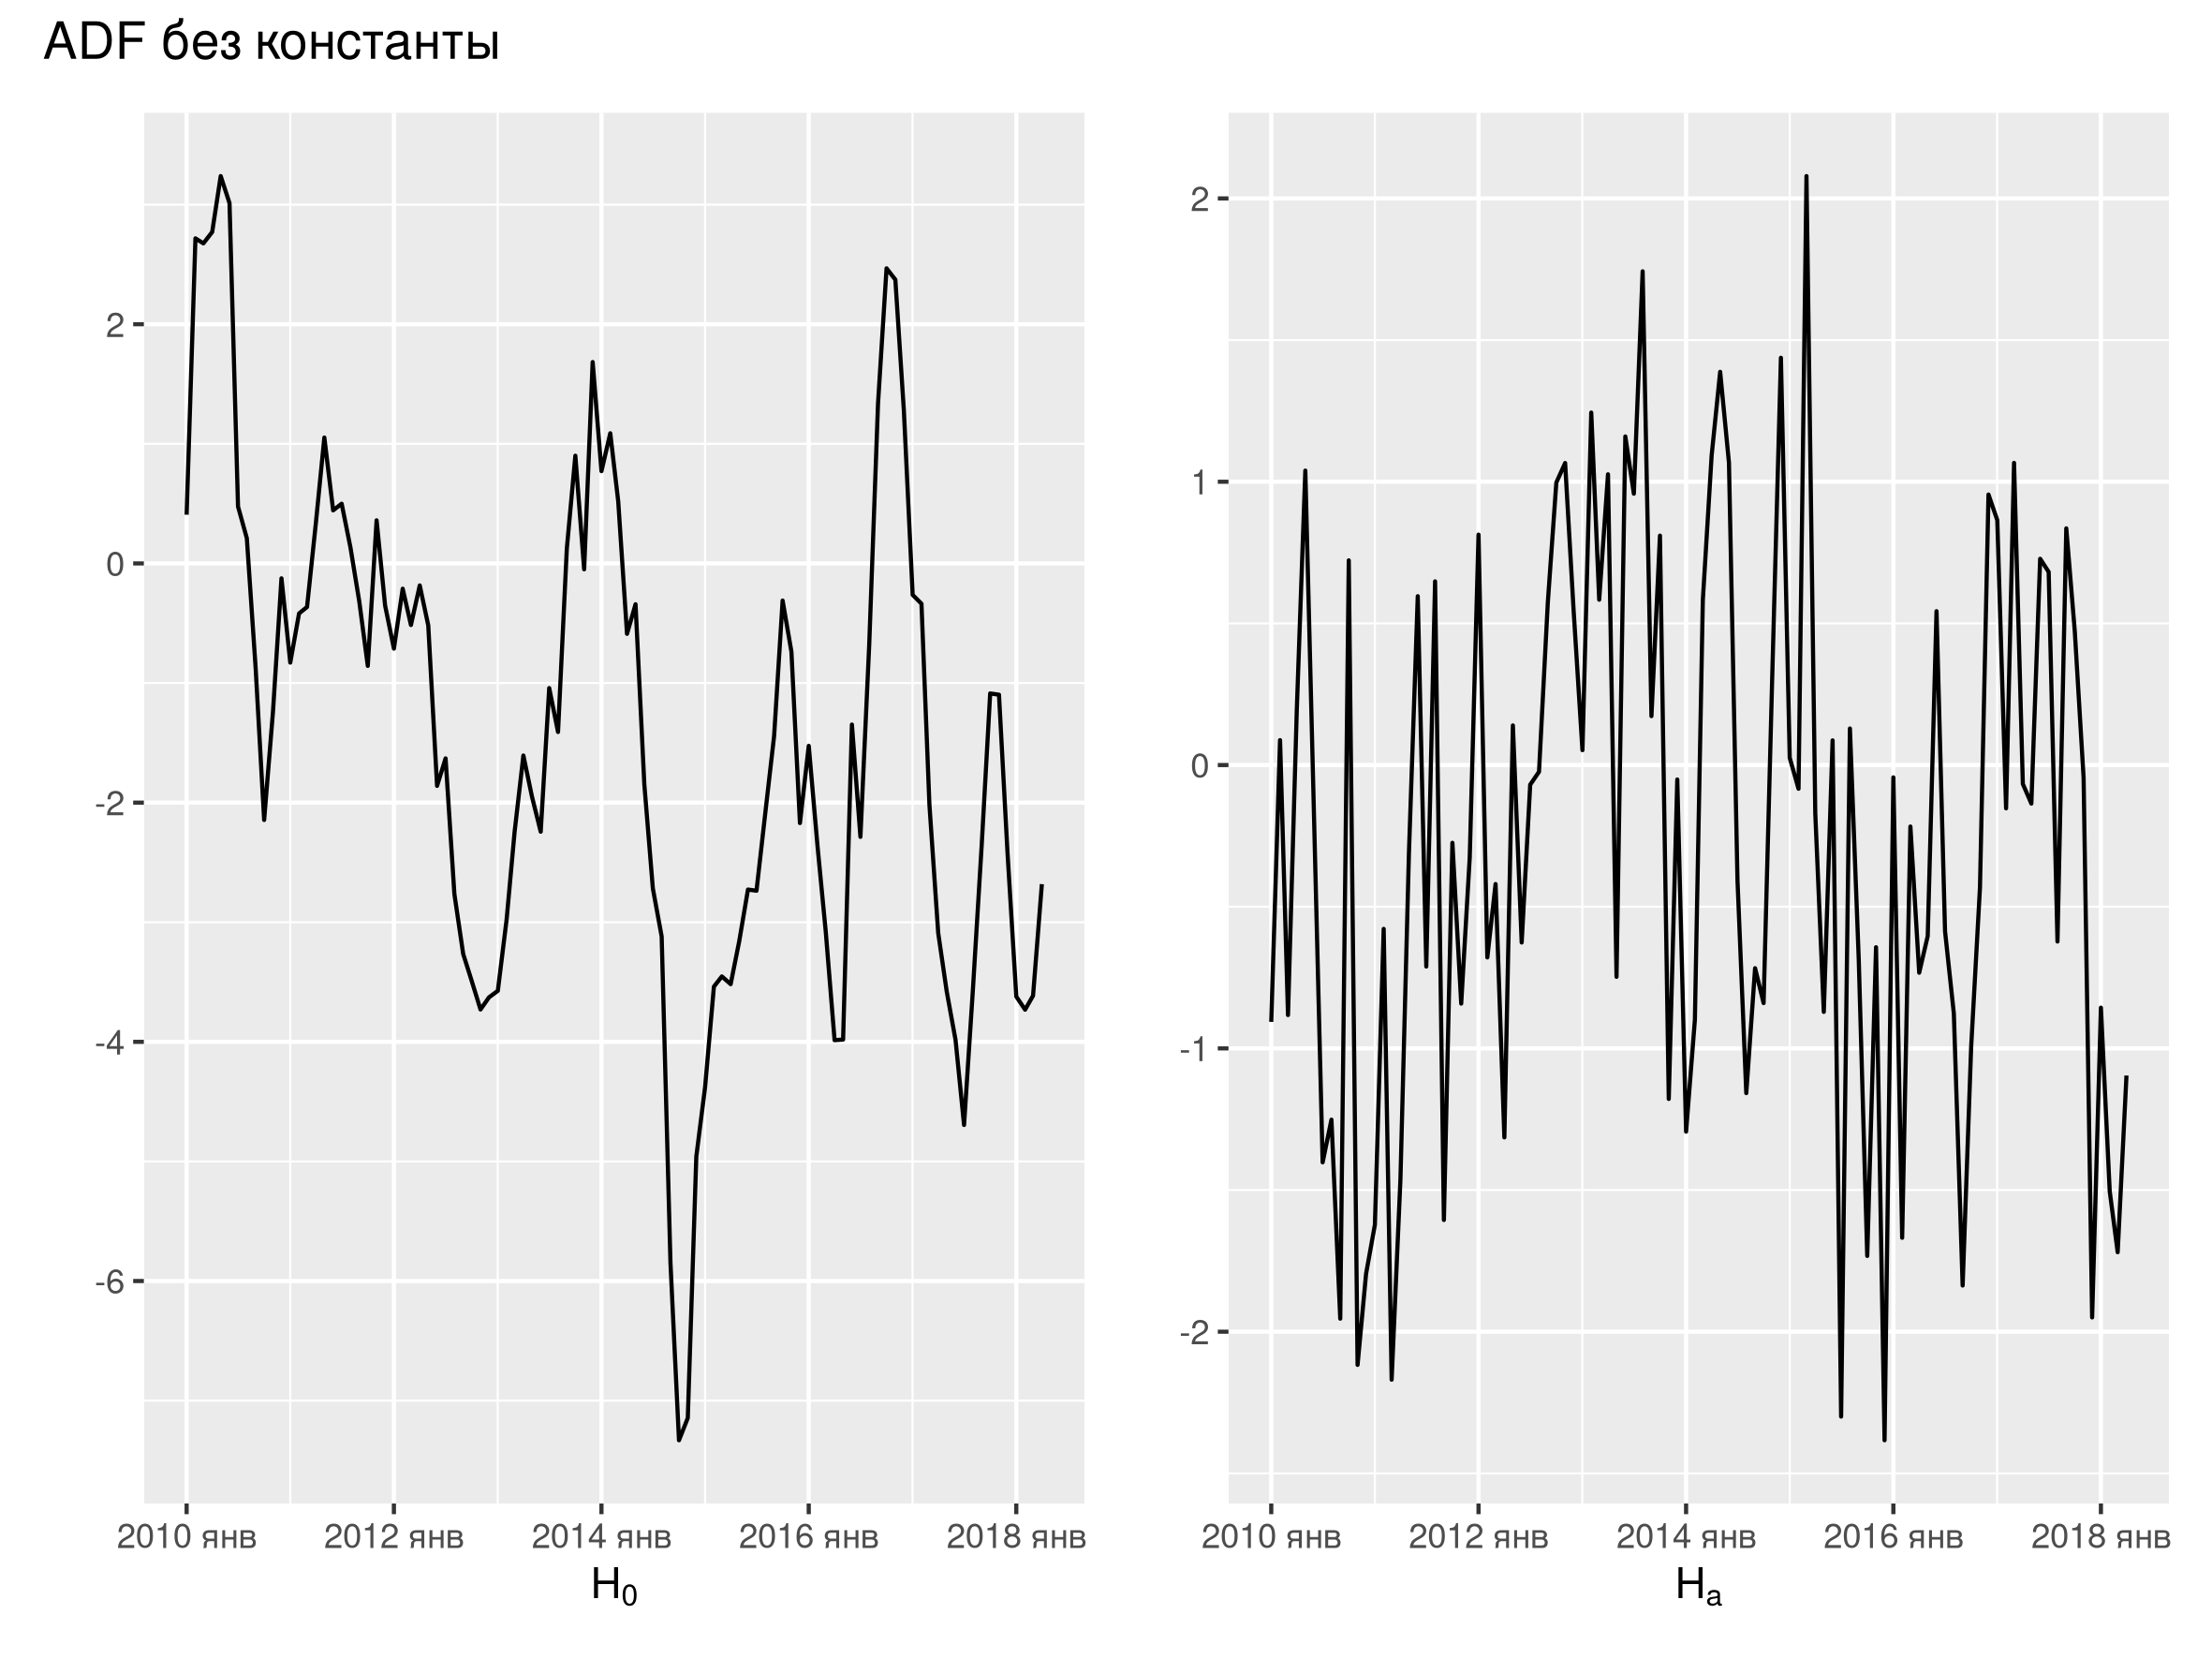
\includegraphics[width=\textwidth]{pictures/om_ts_06-055.png}

\end{frame}



\begin{frame}
  \frametitle{ADF с трендом}
  \[
  \Delta y_t = c + g t + \beta y_{t-1} + d_1 \Delta y_{t-1} + \ldots + d_p \Delta y_{t-p} + u_t,  
  \]

  \pause

  \alert{$H_0$: $\beta = 0$};
  
  $\Delta y_t = k_1 + k_2 t + x_t$;
  
  $(x_t)$ — стационарный $AR(p)$ процесс c $\E(x_t) = 0$;

  $y_t = y_0 + m_1 t + m_2 t^2 + \sum_{i=1}^t x_i$;

  \pause

  \alert{$H_a$: $\beta < 0$};

  $y_t = m_1 + m_2 t + x_t$;
  
  $(x_t)$ — стационарный $AR(p + 1)$ процесс с $\E(x_t) = 0$;

  \pause 

  В алгоритме будет регрессия \alert{с константой и трендом} и другое распределение $DF^{ct}$.

\end{frame}


\begin{frame}
  \frametitle{ADF с трендом: $H_0$ и $H_a$}
  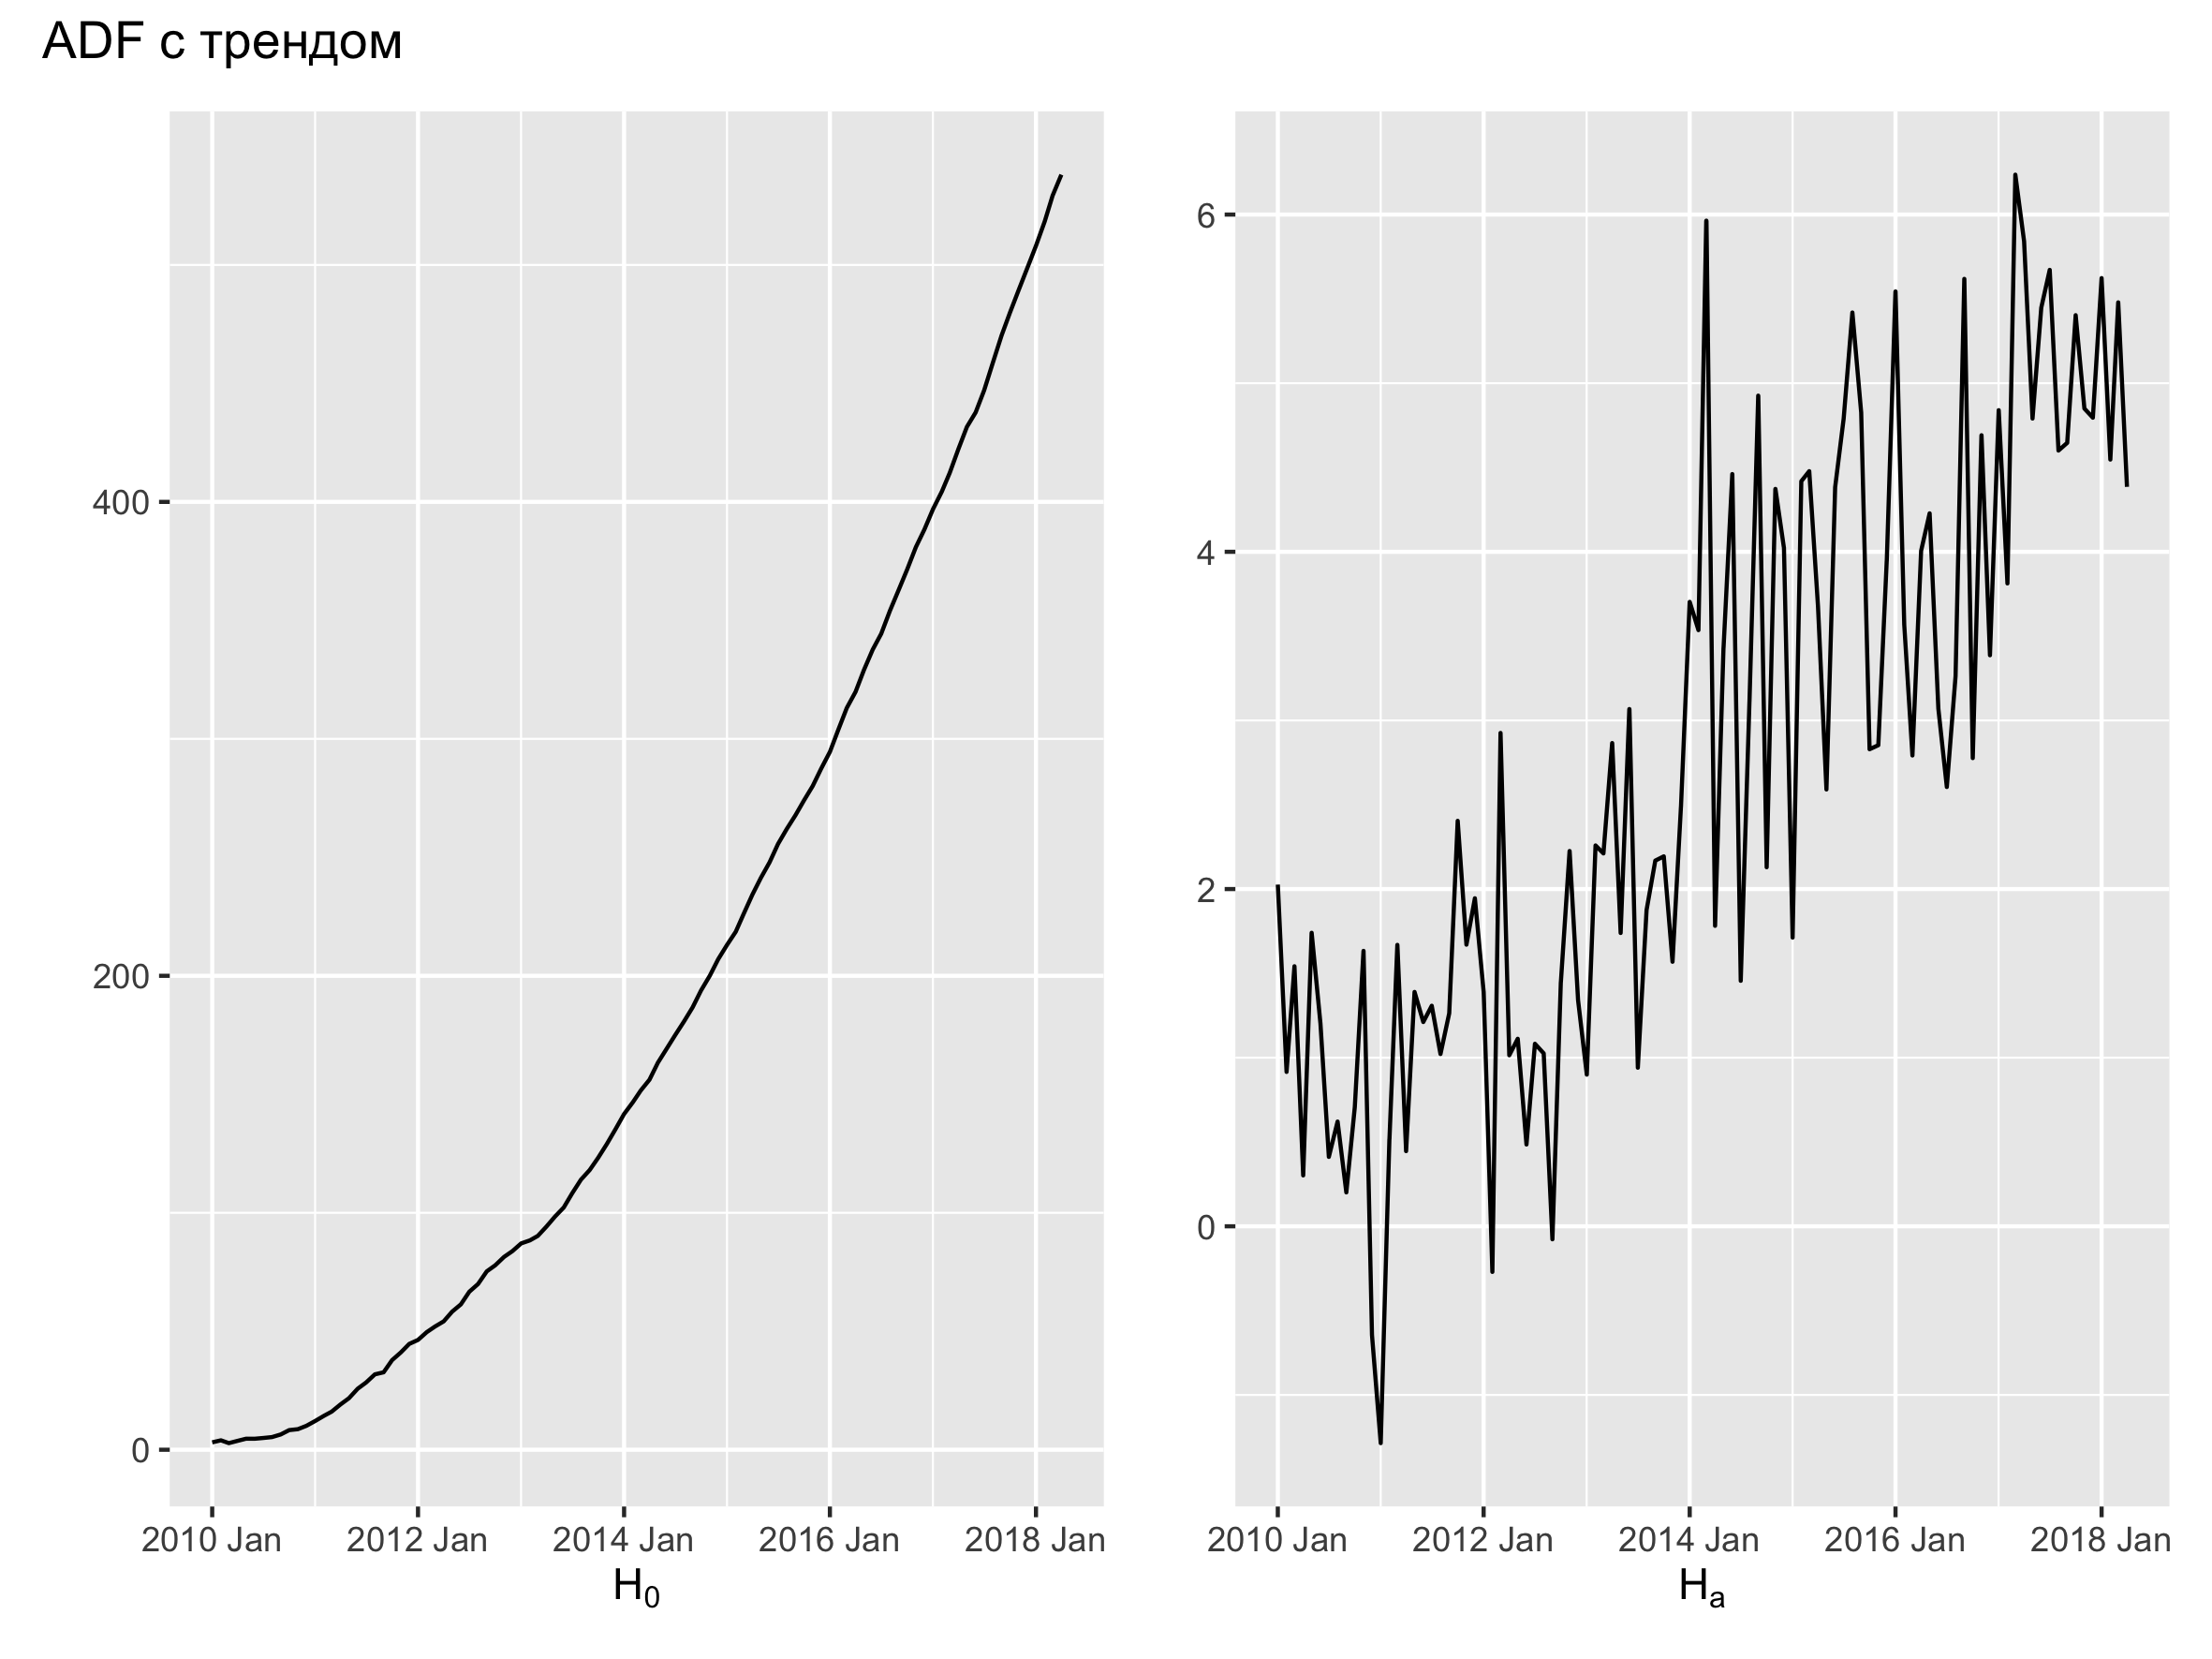
\includegraphics[width=\textwidth]{pictures/om_ts_06-060.png}
\end{frame}


\begin{frame}{$ADF$ тест: итоги}

  \begin{itemize}[<+->]
    \item Применим для принятия решения о переходе к $\Delta y_t$.
    \item Есть три варианта теста с разными предпосылками.
  \end{itemize}
\end{frame}



